\documentclass{beamer}

%\input{embed_video.tex}
\mode<presentation>
{
  \usetheme{Boadilla}
  % possiblities Singapore, Malmoe, Dresden 
  \setbeamercovered{invisible}
}

%\setbeamertemplate{navigation symbols}{} 
% removes the navigation symbols

%color setting more or less matching U of A colors
\setbeamercolor*{palette secondary}{use=structure,fg=white,bg=structure.fg!55!black}
\setbeamercolor*{palette tertiary}{use=structure,fg=white,bg=red!50!black}

\usepackage[english]{babel}
\usepackage{tikz}
\usetikzlibrary{patterns,hobby,snakes}
\usepackage{pgfplots}
\pgfplotsset{compat=1.6}
\usepgfplotslibrary{fillbetween}
\usepackage{tabularx,booktabs}
\usepackage[utf8]{inputenc}
\usepackage[T1]{fontenc}
\usepackage{graphicx}
\usepackage{amsfonts}
\usepackage[
    backend=biber,
    style=phys,
    pageranges=false,
    biblabel=brackets,
    chaptertitle=false,
    articletitle=false,
    maxbibnames=3,
    doi=false, url=false, isbn=false
]{biblatex}
%\usepackage[backend=biber]{biblatex}
\addbibresource{presentation.bib}

\title[TPS free energies]{Transition path sampling and the calculation of free energies of enzymatic reactions}
%\subtitle{} 

\author[Schwartz Group]{Sree Ganesh Balasubramani}

\institute[U of A]{Schwartz Group \\ Chemistry and Biochemistry \\ University of Arizona}
\date{}
% If you wish to uncover everything in a step-wise fashion, uncomment
% the following command: 
%\beamerdefaultoverlayspecification{<+->}
\begin{document}
%------------------------------------------------------------------------------
\begin{frame}
  \titlepage
\end{frame}
%------------------------------------------------------------------------------
\begin{frame}
  \frametitle{Outline}
  \begin{itemize}[<+-|alert@+>]
      \item Motivations
      \item Introduction to transition path sampling 
      \item Equilibrium sampling within TPS
      \item Algorithm 
      \item Results
  \end{itemize}
\end{frame}
%------------------------------------------------------------------------------
%\begin{frame}
%\frametitle{Motivations}
%\begin{block}{Why study enzyme activity?}
%{
%    \begin{itemize}
%        \item Efficient catalysts
%        \item Design transition state analogues and inhibitors
%        \item Directed evolution to obtain more efficient enzymes
%    \end{itemize}
%}
%\end{block}
%\pause
%\begin{block}{Why use molecular dynamics simulations?}
%{
%\begin{itemize}
%    \item Enzyme activity in atomistic detail
%    \item  Hard to probe transition state structures using physical or spectroscopic 
%     methods since they typically have extremely short lifetimes ($10^{-13}\;s$)
% \end{itemize}
%}
%\end{block}
%\end{frame}
%------------------------------------------------------------------------------
\begin{frame}
\frametitle{Motivations: Sampling rare but important events}
\pause
\begin{figure}
\centering
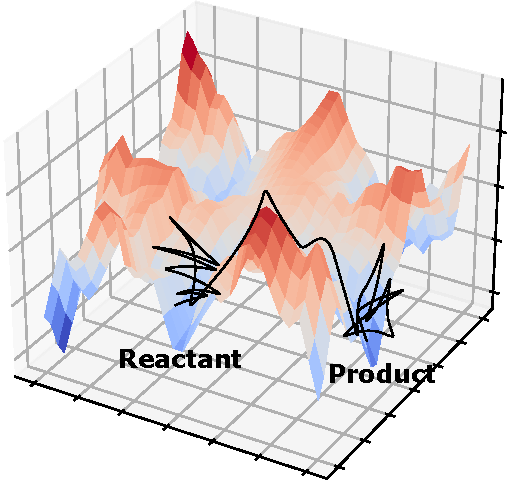
\includegraphics[scale=0.5]{figures/pot-surf.pdf}
\end{figure}
\begin{block}{Time scales in molecular dynamics simulations}
{
    \begin{itemize}
        \item Consider the dissociation of a weak acid in water, with a half life of say $1\;ms$ 
        \item Straightforward MD simulations with $1\;fs$ time step (takes $1\;s$ of wall time to simulate)
        would take $10^{12}\;s$ of wall time to observe a single dissociation event 
    \end{itemize}
}
\end{block}
\end{frame}
%------------------------------------------------------------------------------
\begin{frame}
\frametitle{Enhanced sampling techniques}
\pause
Umbrella sampling, metadynamics, milestoning, conformational flooding, adaptive biasing force method and so on 
\pause
\begin{block}
{
    \begin{itemize}
        \item Rendered MD simulations to be widely applicable in the fields of chemistry, condensed matter physics, biology and materials science
        \pause
        \item Use of predefined reaction coordinates, which can be complicated for large biomolecular systems
        \pause
        \item Use of biasing potential to access regions in phase space with high free energy barriers
    \end{itemize}
}
\end{block}
\end{frame}
%------------------------------------------------------------------------------
\begin{frame}
\frametitle{Transition path sampling (TPS)\footfullcite{Bolhuis02AnnRevPhysChem53p291}}
\pause
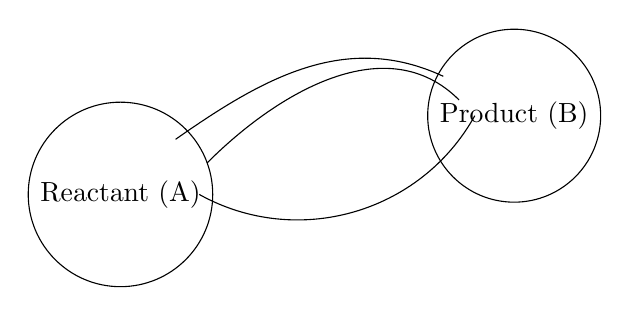
\begin{tikzpicture}
  [every rectangle node/.style={draw},
   every circle node/.style={draw}]
  \draw (0,0) node[circle] {Reactant (A)}; 
  \draw (5,1) node[circle] {Product (B)};
    %\draw[snake=coil,segment aspect=0,red,thick] (0,0) node[circle] {Reactant (A)} -- (4,1) node[circle] {Product (B)};
    %\draw (0.3,0) arc (180:90:3cm) -- (3.7,1.3) arc (90:0:1cm);
    %\draw (0.3,0) arc (180:90:3cm) -- (3.7,1.3);
    \pause
    \draw[yshift=0cm]  (1,0) to [bend right=45] (4.5,1);
    \pause
    \draw[yshift=0cm]  (1.1,0.4) to [out=45, in=135] (4.3,1.2);
    \pause
    \draw[yshift=0cm]  (0.7,0.7) to [out=35, in=155] (4.1,1.5);
    %\draw (0.3,0.2) arc (160:80:1cm) -- (3.5,1.5) arc (97:0:1cm);
\end{tikzpicture}
\begin{block}
{
    \begin{itemize}
        \item Focus on pathways connecting long lived reactant and product states 
        \item Reaction coordinate and bias potential free description
        \item Monte Carlo algorithm that is easy to implement
        \item Transition state, reaction coordinates, kinetic parameters
    \end{itemize}
}
\end{block}
\end{frame}
%------------------------------------------------------------------------------
\begin{frame}
\frametitle{Trajectories in phase space}
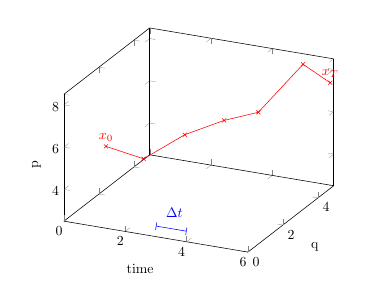
\begin{tikzpicture}[scale=0.5]
\begin{axis}[
    %y label style={rotate=45, anchor=south west},
    xlabel=time,
    ylabel=q,
    zlabel=p]
  \addplot3[color=red,mark=x,point meta=explicit symbolic,nodes near coords] coordinates {
    (0.0,2.4,4.5)[$x_0$]
    (1.0,2.8,3.9)
    (2.0,3.4,4.9)
    (3.0,3.9,5.5)
    (4.0,4.1,6.0)
    (5.0,4.9,8.0)
    (6.0,4.7,7.5)[$x_{T}$]
  };
  \addplot3[color=blue,|-|] coordinates{ (3,0.0,3.0) (4,0.0,3.0)}%;
  node[above] at (axis cs:3.6,0.0,3.3) {$\Delta t$};
  %\node[] at (1.5,2.0,.5) {$\Delta t$};
  \end{axis}
\end{tikzpicture}
%
%\newline
\begin{block}{Definitions}
{
\begin{itemize}
\item $x_0$: initial state, $T:$ time length of trajecotry, $\Delta t:$ time step, $x_{i\Delta t}:$ time slice ($i\in \{0,1,\ldots\}$)
\item $x = \{\vec{q},\vec{p}\}$ where $\vec{q}:$ generalized coordinates and $\vec{p}:$ generalized momenta 
\end{itemize}
}
\end{block} 
\end{frame}
%------------------------------------------------------------------------------
\begin{frame}
\frametitle{Monte Carlo in path space: the shooting algorithm}
%\begin{block}
\begin{itemize}
    \item Start with an initial biased reactive trajectory
\end{itemize}
%\end{block}
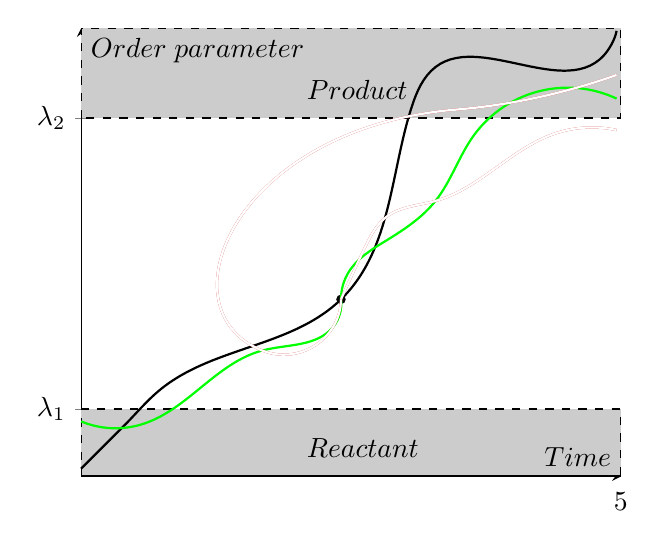
\begin{tikzpicture}
 \begin{axis}[
        xmin=0.0,xmax=5.0,
        ymin=0,ymax=5.0,
        xtick={0.0, 5.0},
        %xticklabels={$v_1$,$v_2$},
        ytick={0.75,4.0},
        yticklabels={$\lambda_1$,$\lambda_2$},
        xlabel={$Time$},  
        ylabel={$Order\;parameter$},
        every axis x label/.style={
    at={(ticklabel* cs:5.05)},
    anchor=west,
},
every axis y label/.style={
    at={(ticklabel* cs:5.05)},
    anchor=south,
},
        axis lines=middle] 
    \draw [fill=gray!40!white,thick,dashed] (axis cs:0,0) rectangle (axis cs:5.0,0.75);
    \draw [fill=gray!40!white,thick,dashed] (axis cs:0,4.0) rectangle (axis cs:5.0,5.0);
    \addplot+[black,thick,domain=0:5,no marks] {0};
    %
    \node  at (axis cs:2.0,4.1)    [anchor=south west] {$Product$};
    \node  at (axis cs:2.0,0.1)    [anchor=south west] {$Reactant$};
    \end{axis}
\pause
\draw [thick] (0.0 ,0.1)  to [ curve through ={(0.5, 0.6) . . (0.55, 0.65)  . . (1.0,1.1) . . (3.3, 2.25) . . (4.2, 4.7) . . (4.5,5.2) . . (6.77, 5.56)  }] (6.8,5.66) ;% curve 
\pause
\filldraw (3.3,2.25) circle[radius=1.5pt];
\pause
\draw [green,thick] (3.3 ,2.25) to [ curve through ={(3.4,2.6)  . . (3.88, 3.00) . . (4.5,3.5) . . (5.0,4.35)  }] (6.8,4.8);% curve
\pause  
\draw [green,thick] (3.3 ,2.25) to [ curve through ={(3.2,1.9)  . . (2.3,1.6) . . (0.76,0.66)  }] (0.0,0.7);% curve 
\pause
\draw [gray!40!red,thick] (3.3 ,2.25) to [ curve through ={(3.6,2.9)  . . (3.88, 3.30) . . (4.5,3.5) . . (6.0,4.35)  }] (6.8,4.4);% curve
\pause  
\draw [gray!40!red,thick] (3.3 ,2.25) to [ curve through ={(3.2,1.9)  . . (2.3,1.6) . . (4.76,4.66)  }] (6.8,5.1);% curve 
\pause
\draw [white,thick] (3.3 ,2.25) to [ curve through ={(3.6,2.9)  . . (3.88, 3.30) . . (4.5,3.5) . . (6.0,4.35)  }] (6.8,4.4);% curve
\pause  
\draw [white,thick] (3.3 ,2.25) to [ curve through ={(3.2,1.9)  . . (2.3,1.6) . . (4.76,4.66)  }] (6.8,5.1);% curve 
\end{tikzpicture}
\end{frame}
%------------------------------------------------------------------------------
\begin{frame}
\frametitle{Separatrix and committor analysis\footfullcite{Dellago2006}}
\begin{figure}
\centering 
\includegraphics[scale=0.4]{figures/separatrix-full.png}
\caption{The probability of trajectories started from a time slice to reach the reactant ($P_A$) and the product $P_B$
are equal for the transition state}
\end{figure}
\end{frame}
%------------------------------------------------------------------------------
\begin{frame}
\frametitle{TPS ensemble}
Pathways connecting $\mathcal{A}$ and $\mathcal{B}$ in phase space have an associated probability distribution of
\begin{equation}
\mathcal{P}_{\mathcal{AB}}[x_{\mathcal{T}}] = h_{\mathcal{A}}(x_0)\mathcal{P}[x(\mathcal{T})]
h_{\mathcal{B}}(x_{\mathcal{T}})/Z_{\mathcal{AB}}(\mathcal{T})\label{eqn:tpsensem}\nonumber 
\end{equation}
where 
\[
    h_{\mathcal{A}/\mathcal{B}}(x)= 
\begin{cases}
    1, & \text{if } x\in \mathcal{A}/\mathcal{B}\\
    0,              & \text{otherwise}
\end{cases}
\]
and $Z_{\mathcal{AB}}(\mathcal{T})$ is the normalization factor for this 
probability distribution function.
\begin{block}{}
At equilibrium the distribution of pathways is different as transition pathways undersample the 
regions $\mathcal{A}$ and $\mathcal{B}$
\end{block}
\end{frame}
%------------------------------------------------------------------------------
%\begin{frame}
%\frametitle{Equilibrium sampling in trajectory space}
%
%\end{frame}
%------------------------------------------------------------------------------
\begin{frame}
\frametitle{Equilibrium sampling in trajectory space: The algorithm}
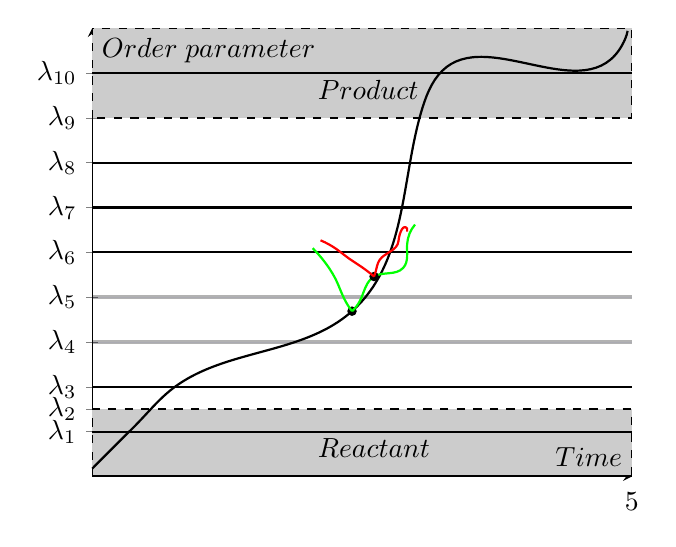
\begin{tikzpicture}
%\draw [thick] (0.0 ,0.1) to [ curve through ={(0.5, 0.6) . . (0.55, 0.65)  . . (1.0,1.1) . . (3.3, 2.25) . . (4.2, 4.7) . . (4.5,5.2) . . (6.77, 5.56)  }] (6.8,5.66);%
\pause
 \begin{axis}[
        xmin=0.0,xmax=5.0,
        ymin=0,ymax=5.0,
        xtick={0.0, 5.0},
        %xticklabels={$v_1$,$v_2$},
        ytick={0.5,0.75,1.0,1.5,2.0,2.5,3.0,3.5,4.0,4.5},
        yticklabels={$\lambda_1$,$\lambda_2$,$\lambda_3$,$\lambda_4$,$\lambda_5$,$\lambda_6$,$\lambda_7$,$\lambda_8$,$\lambda_9$,$\lambda_{10}$},
        xlabel={$Time$},  
        ylabel={$Order\;parameter$},
        every axis x label/.style={
    at={(ticklabel* cs:5.05)},
    anchor=west,
},
every axis y label/.style={
    at={(ticklabel* cs:5.05)},
    anchor=south,
},
        axis lines=middle] 
    \draw [fill=gray!40!white,thick,dashed] (axis cs:0,0) rectangle (axis cs:5.0,0.75);
    \draw [fill=gray!40!white,thick,dashed] (axis cs:0,4.0) rectangle (axis cs:5.0,5.0);
    \draw [fill=gray!40!white,thick,dashed] (axis cs:0,0.5) rectangle (axis cs:5.0,0.5);
    \draw [fill=gray!40!white,thick,dashed] (axis cs:0,1.0) rectangle (axis cs:5.0,1.0);
    %\draw [fill=blue,ultra thick,opacity=0.3] (axis cs:0,1.5) rectangle (axis cs:5.0,1.5);
    \draw [fill=blue,ultra thick,opacity=0.3] (axis cs:0,1.5) -- (axis cs:5.0,1.5);
    \draw [fill=blue,ultra thick,opacity=0.3] (axis cs:0,2.0) rectangle (axis cs:5.0,2.0);

    \draw [fill=gray!40!white,thick,dashed] (axis cs:0,2.5) rectangle (axis cs:5.0,2.5);
    \draw [fill=gray!40!white,thick,dashed] (axis cs:0,3.0) rectangle (axis cs:5.0,3.0);
    \draw [fill=gray!40!white,thick,dashed] (axis cs:0,3.5) rectangle (axis cs:5.0,3.5);
    \draw [fill=gray!40!white,thick,dashed] (axis cs:0,4.5) rectangle (axis cs:5.0,4.5);
    \addplot+[black,thick,domain=0:5,no marks] {0};
    %
    \node  at (axis cs:2.0,4.1)    [anchor=south west] {$Product$};
    \node  at (axis cs:2.0,0.1)    [anchor=south west] {$Reactant$};
    \end{axis}
    %\draw [thick] (0.0 ,0.1) to [ curve through ={(0.5, 0.6) . . (0.55, 0.65)  . . (1.0,1.1) . . (3.3, 2.1) . . (4.2, 4.7) . . (4.5,5.2) . . (6.77, 5.56)  }] (6.8,5.66);% curve
    \draw [thick] (0.0 ,0.1) to [ curve through ={(0.5, 0.6) . . (0.55, 0.65)  . . (1.0,1.1) . . (3.3, 2.1) . . (4.2, 4.7) . . (4.5,5.2) . . (6.77, 5.56)  }] (6.8,5.66);% curve
    \pause
    \filldraw (3.3,2.1) circle[radius=1.5pt];
    \pause
    \draw [green,thick] (3.3 ,2.1) to [ curve through ={(3.4,2.23)  . . (3.58, 2.54) . . (3.95,2.65) . . (4.0,2.95)  }] (4.1,3.2);% curve
    \pause  
    \draw [green,thick] (3.3 ,2.1) to [ curve through ={(3.2,2.26)  . . (3.1,2.49) . . (3.0,2.66)  }] (2.8,2.9);% curve 
    \pause
    \filldraw (3.58,2.54) circle[radius=1.5pt];
    \pause
    \draw [red,thick] (3.58 ,2.54) to [ curve through ={(3.6,2.6)  . . (3.65, 2.75) . . (3.89,2.99) . . (4.0,3.15)  }] (4.0,3.11);% curve
    \pause
    \draw [red,thick] (3.58 ,2.54) to [ curve through ={(3.48,2.62)  . . (3.38, 2.69) . . (3.26,2.77) . . (3.1,2.89)  }] (2.9,3.0);% curve
\end{tikzpicture}
\end{frame}
%------------------------------------------------------------------------------
\begin{frame}
\frametitle{Free energies from TPS}
\begin{equation}
A[\lambda_i] = -k_BTlog(P(\lambda_i)) +\;\text{constant} \nonumber 
\end{equation}
The probability of $P(\lambda_i)$ is defined by
\begin{equation}
P(\lambda_i) = \int \textbf{dV} \rho({\vec{q}})\delta(\lambda_i-\tilde{\lambda}(\vec{q})) \nonumber 
\end{equation}
In practice, the calculation of $P(\lambda_i)$ proceeds through histogram based techniques. 
\end{frame}
%------------------------------------------------------------------------------
\begin{frame}
\frametitle{QM/MM simulations}
CHARMM force field consists of intramolecular terms such as 
\begin{align}
E_{int} = &\sum_{bonds}k_r(r-r_{0})^2 + \sum_{angles}k_{\theta}(\theta - \theta_{0})^2 \nonumber \\ &+ \sum_{dihedrals}k_{\phi}(1+\cos(n\phi-\delta)) \nonumber \\
&+ \sum_{imp.\;dihed.} k_{\psi}(\psi - \psi_0)^2 + \sum_{Urey-Bradley} k_{\text{UB}}(r_{1,3}-r_{1,3;0}) \nonumber 
\end{align}\pause
and intermolecular terms such as 
\begin{align}
\sum_{nonbonded} \left(\frac{q_iq_j}{4\pi\epsilon r_{ij}} - E_{min} 
\left[\left(\frac{R_{min}}{r_{ij}}\right)^{12} - \left(\frac{R_{min}}{r_{ij}}\right)^{6} \right] \right)\nonumber 
\end{align}
\end{frame}
%------------------------------------------------------------------------------
\begin{frame}
\frametitle{}
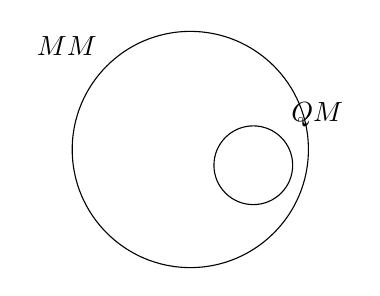
\begin{tikzpicture}
\node [draw,
    circle,
    minimum size =3cm,
    label={135:$MM$}] (A) at (0,0){};
 
% Set B
\node [draw,
    circle,
    minimum size =1cm,
    label={45:$QM$}] (B) at (0.8,-0.2){};
\end{tikzpicture}
\newline
QM methods: semiempirical (PM3, AM1, etc.), density functional approximations ($\mathcal{O}(N^3)$) \\
Stitch the QM and MM regions together with generalized hybrid orbital (GHO) scheme 
\end{frame}
%------------------------------------------------------------------------------
\begin{frame}
\frametitle{Human adenosyl methionine enzyme}
\begin{figure}
\centering 
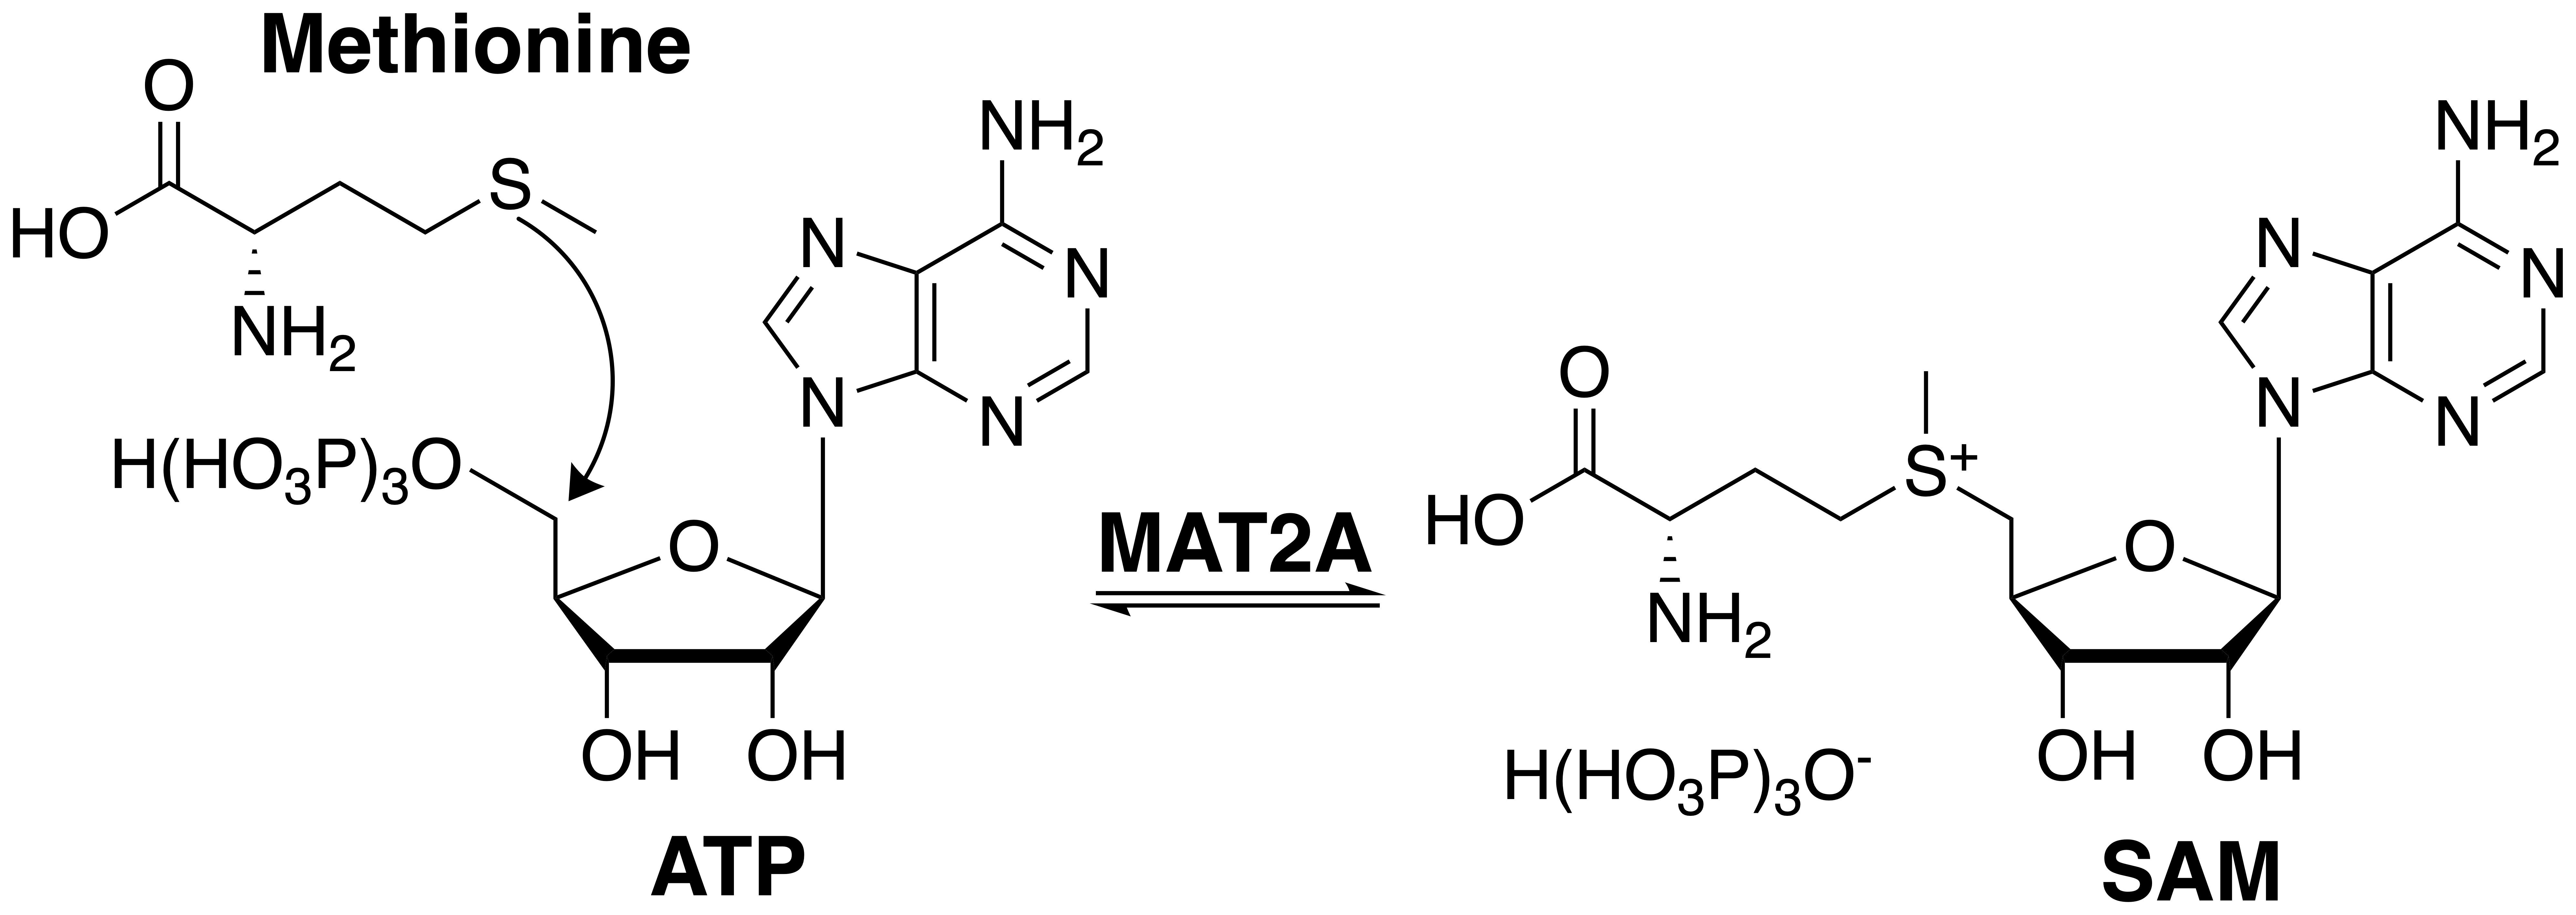
\includegraphics[scale=0.6]{figures/mat2a-reaction.png}
\end{figure}
SAM is an essential metabolite which is distributed to almost all body tissues and fluids, is a
universal methyl donor, and is of fundamental importance to
the metabolism of compounds such as hormones, neurotransmitters, proteins, and nucleic acids.
\end{frame}
%------------------------------------------------------------------------------
\begin{frame}
\frametitle{System preparation}
\begin{itemize}
\item The energies of both the systems were minimized using 50 steps of the 
steepest descent method, followed by 2000 steps of the
adopted basis Newton-Raphson method where only classical molecular mechanics 
was used for the dynamics. 

\item The minimized systems were
heated slowly to 300 K for 35 ps beginning with harmonic
constraints on all atoms except on the H atoms and the TIP3P 
water molecules with gradual reduction of the restraint forces. 

\item 15 ps of equilibration was carried out starting with harmonic 
restraint forces followed by 20 ps of constraint free 
equilibration to prepare the systems for TPS simulations. 

\end{itemize}
\end{frame}
%------------------------------------------------------------------------------
\begin{frame}
\frametitle{System preparation}
\begin{figure}
\centering 
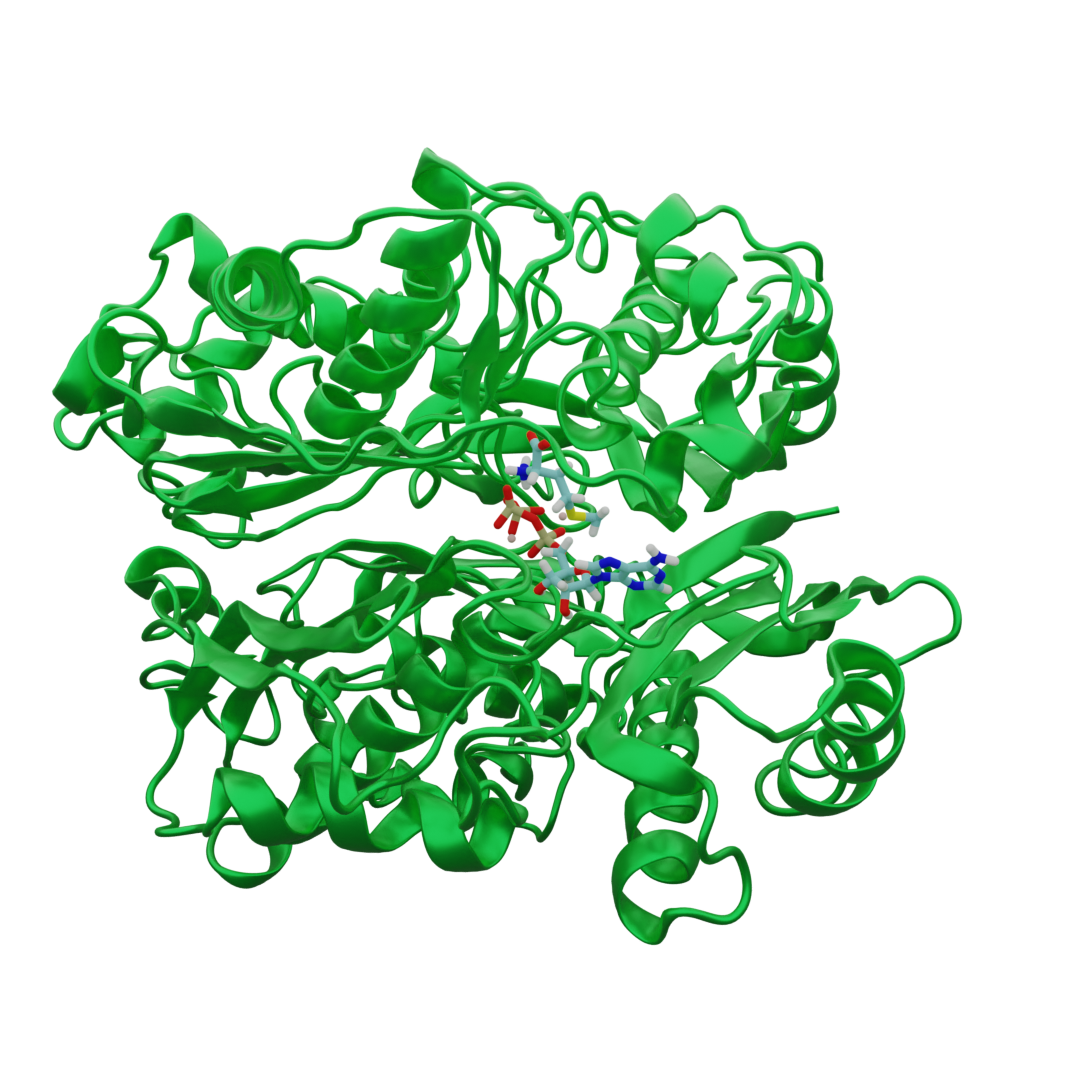
\includegraphics[scale=0.2]{figures/mat2a-equil.png}
\end{figure}
\end{frame}
%------------------------------------------------------------------------------
\begin{frame}
\frametitle{Committor analysis and transition state}
\begin{figure}
\centering
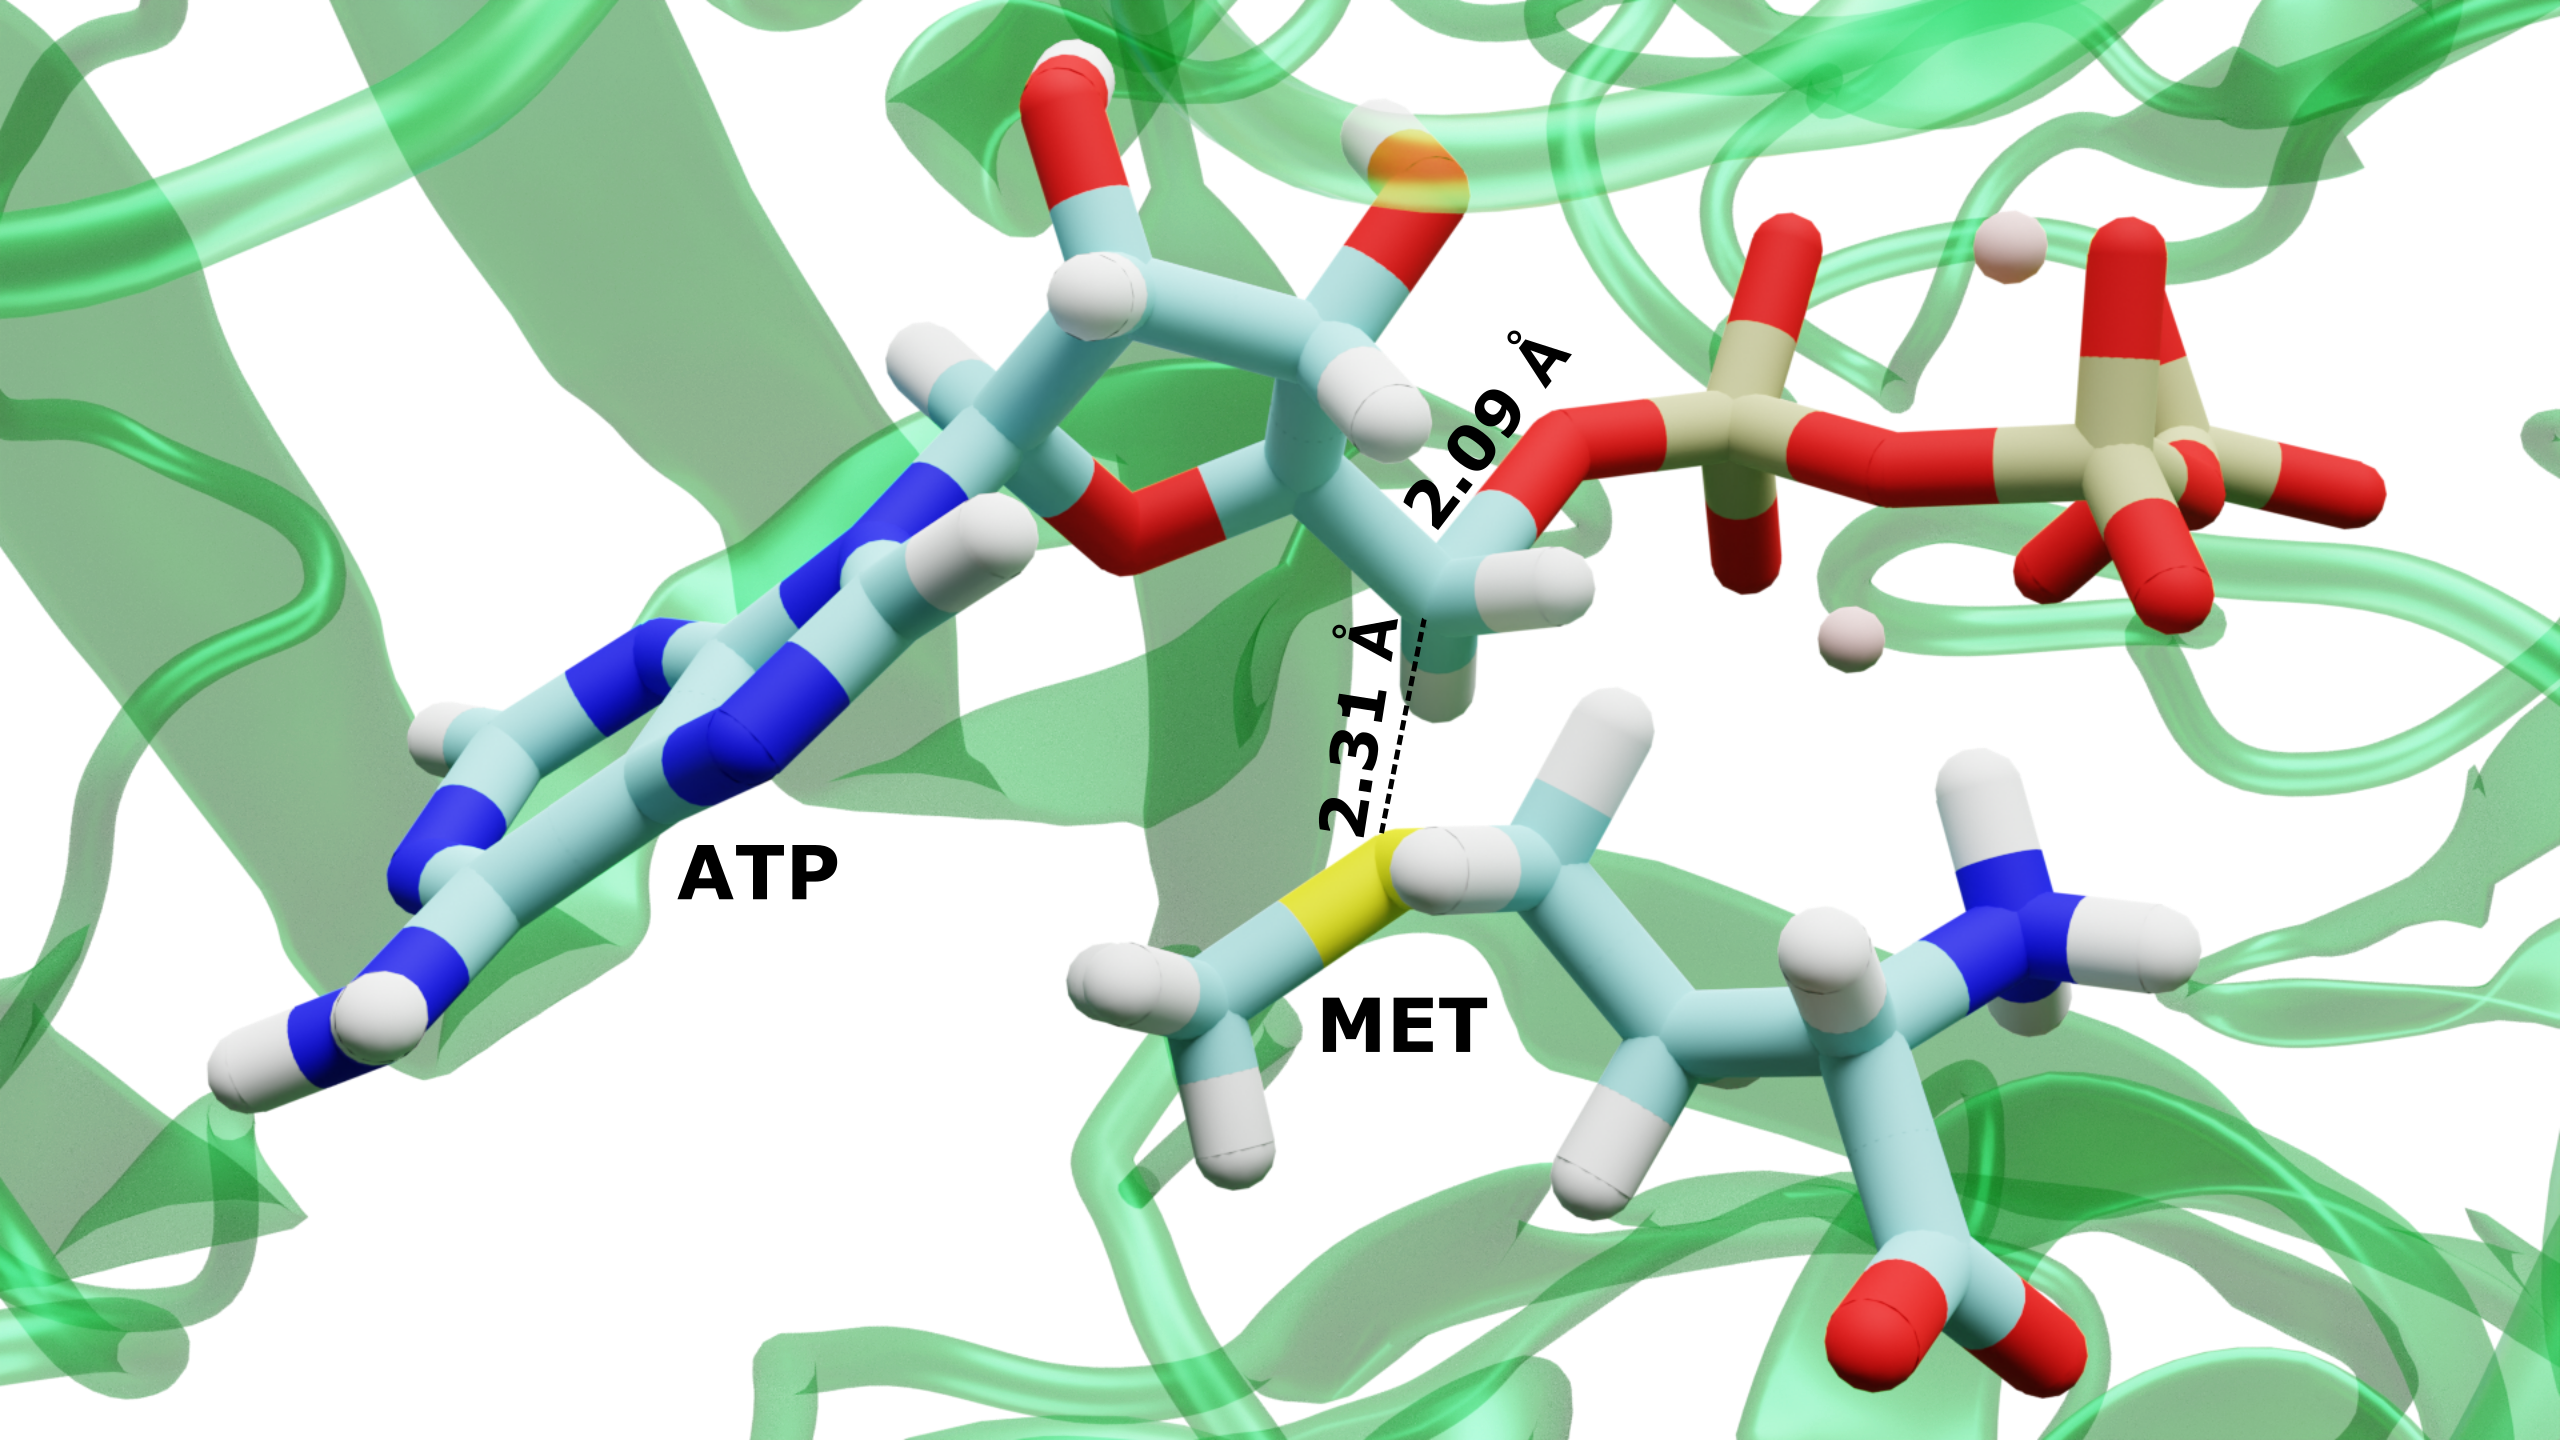
\includegraphics[scale=0.1]{figures/mat2a-trans-labelled.png}
\end{figure}
\begin{center}
\begin{tabular}{l c c}
\hline\hline
 & d$_{\text{SC}}$ ({\AA}) & d$_{\text{OC}}$ ({\AA})\\
\hline
%1 & 2.30 & 2.10 \\
%2 & 2.31 & 2.08 \\
%3 & 2.31 & 2.09 \\
%4 & 2.34 & 2.14 \\
%5 & 2.35 & 2.17 \\
%6 & 2.41 & 2.16 \\
%7 & 2.41 & 2.11 \\
%8 & 2.40 & 2.15 \\
%9 & 2.35 & 2.13 \\
%10& 2.38 & 2.12 \\
%11& 2.29 & 2.06 \\
Mean & 2.35 & 2.12 \\
Stddev & 0.04 & 0.03 \\
\hline\hline
\end{tabular}
\end{center}
Experimental results: $d_{\text{SC}}:\;2.03$ {\AA} and $d_{\text{OC}}:\;2.32$ {\AA}
\end{frame}
%------------------------------------------------------------------------------
\begin{frame}
\frametitle{Committor distribution analysis}
\begin{figure}[ht!]
\centering
\begin{minipage}[b]{0.45\linewidth}
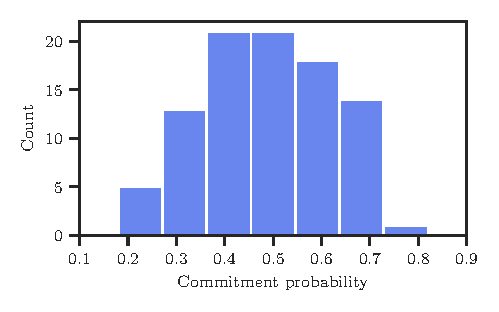
\includegraphics[width=\textwidth]{figures/comm-60-mat2a-nocons.pdf}
\label{fig:minipage1}
\end{minipage}
\quad
\begin{minipage}[b]{0.45\linewidth}
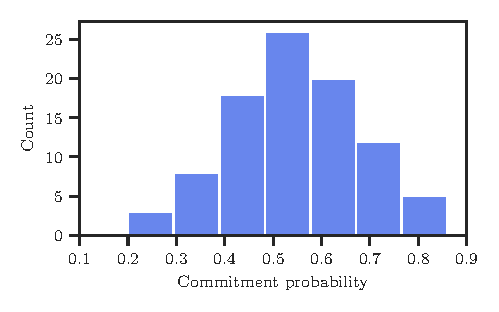
\includegraphics[width=\textwidth]{figures/comm-60-mat2a.pdf}
\label{fig:minipage2}
\end{minipage}
\caption{Committor distribution analysis for obtaining the reaction coordinate of the 
MAT2A catalyzed reaction. The figure on the left has the QM region constrained and the figure 
on the right has the QM region along with the Gln113, Ser114, Arg249 and Arg264 residues constrained.}
\label{fig:mat2a-comm-dist}
\end{figure}
\end{frame}
%------------------------------------------------------------------------------
\begin{frame}
\frametitle{Free energies}
\begin{itemize}
\item 20 overlapping windows, 2500 trajectories of $20\;fs$ length in each window
\end{itemize}
%
\begin{figure}
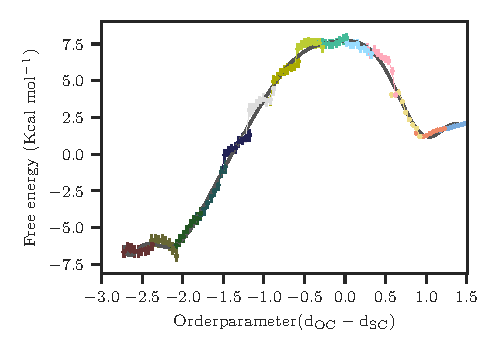
\includegraphics[scale=0.7]{figures/mat2a-fenergy.pdf}
%\caption{Calculated free energy barrier: $16\;kcal\;mol^{-1}$, experimental free energy barrier}
\end{figure}
%
\begin{center}
\begin{tabular}{l c}
\hline\hline
             & Free energy barrier ($kcal\;mol^{-1}$) \\
             \hline
Experimental & 17.27 \\
Calculated & 16\footfullcite{Balasubramani22JPhysChemB126p5413} \\
\hline\hline
\end{tabular}
\end{center}
\end{frame}
%------------------------------------------------------------------------------
\begin{frame}
\frametitle{\textit{Plasmodium vivax} adenosine deaminase}
\begin{figure}
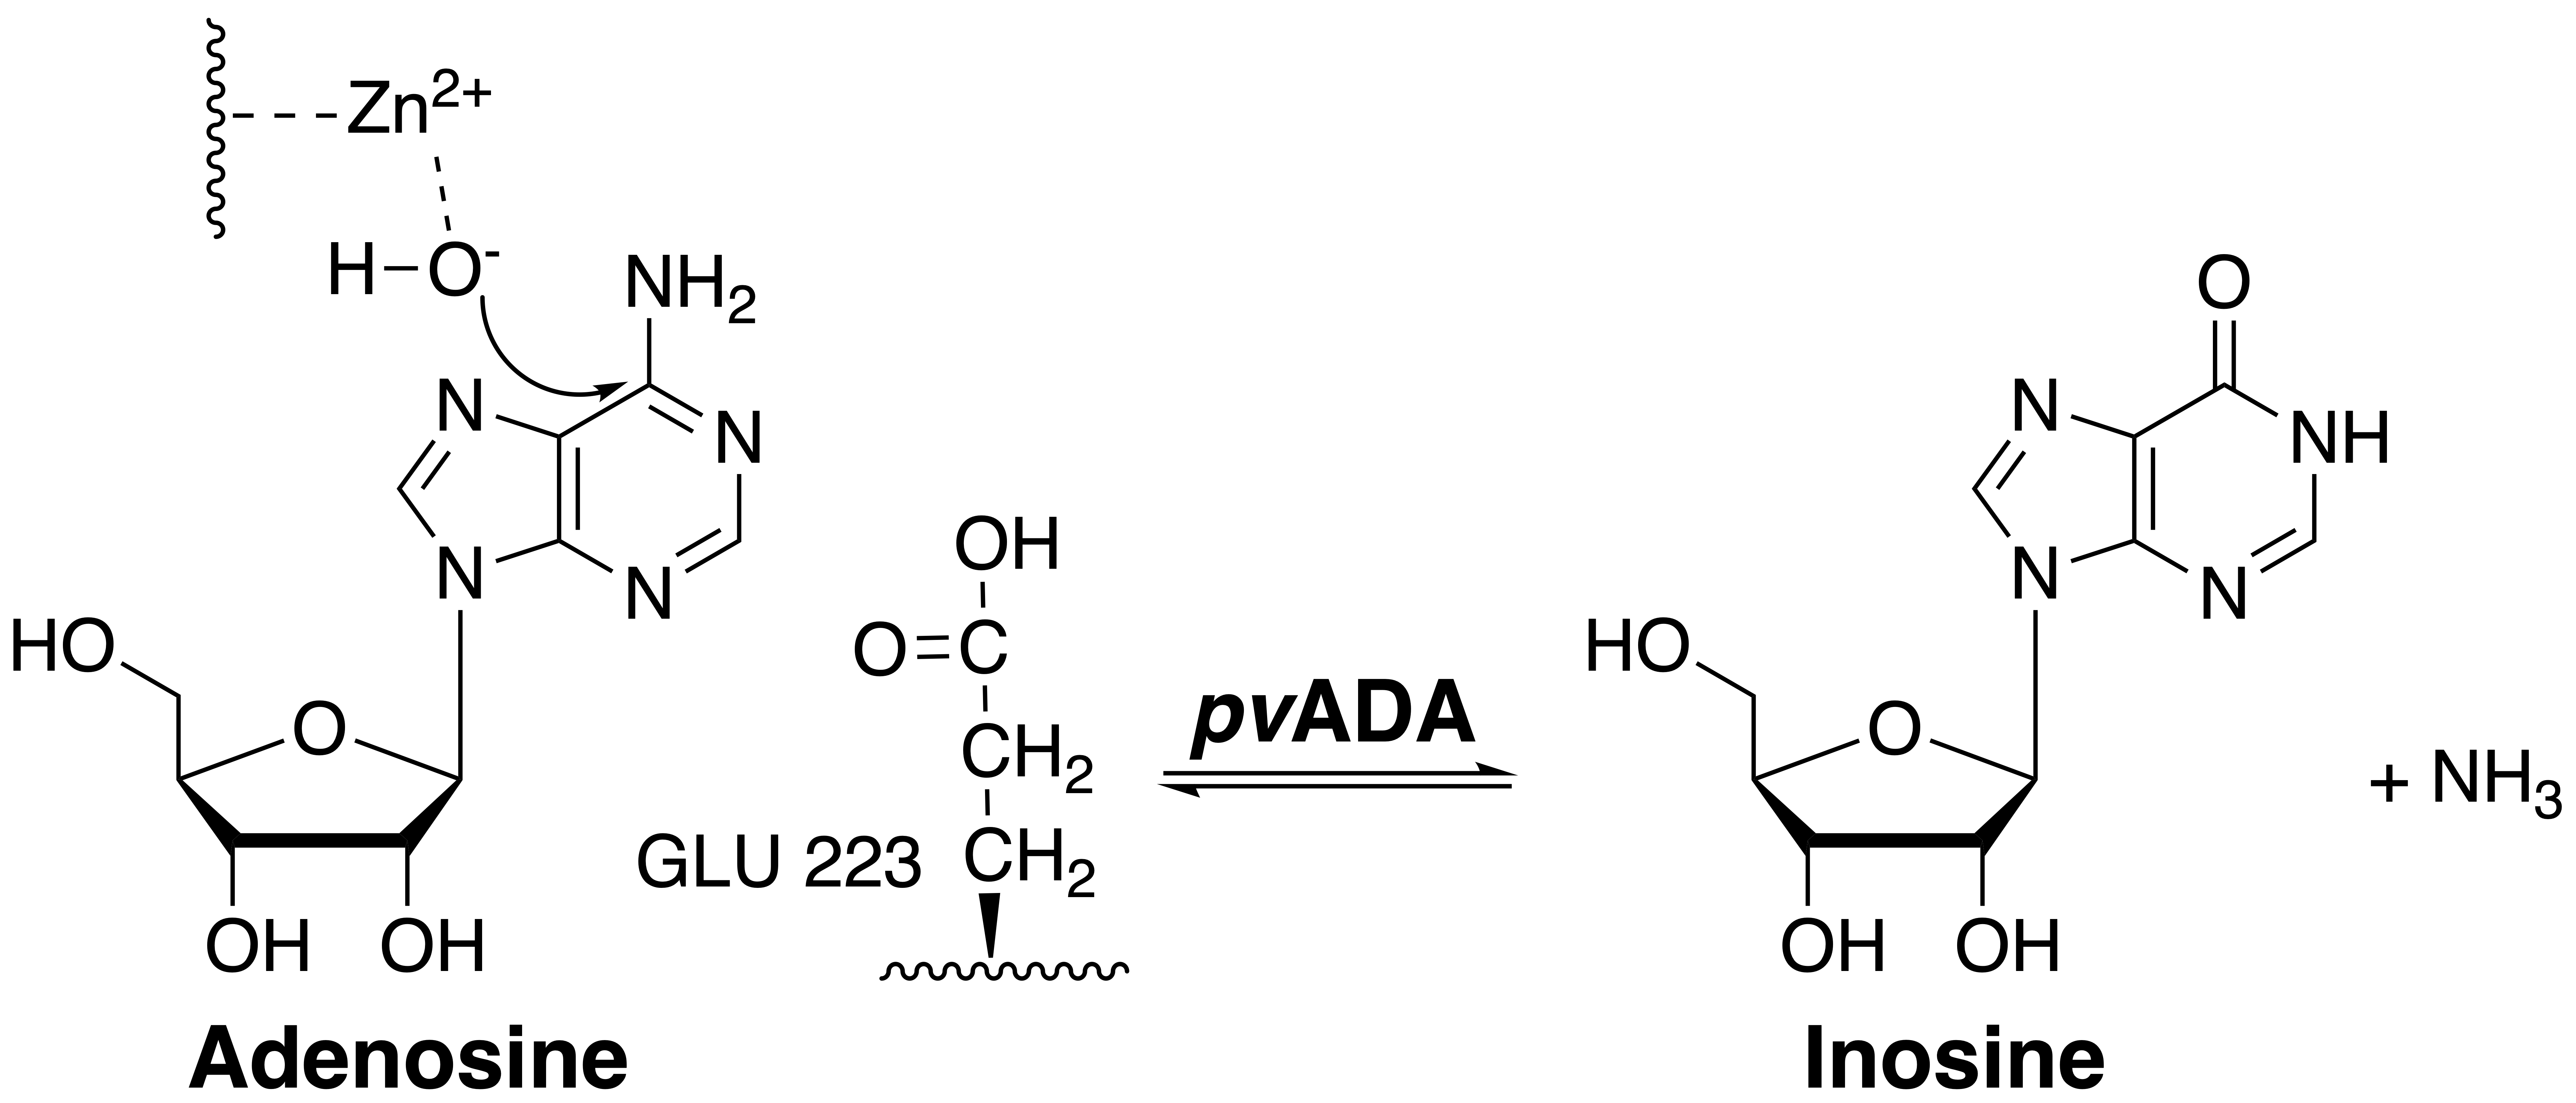
\includegraphics[scale=0.6]{figures/ada-reaction.png}
\end{figure}
\textit{Plasmodium vivax} is a parasite that is responsible for the largest number of cases of
malaria globally
\end{frame}
%------------------------------------------------------------------------------
\begin{frame}
\frametitle{Equilibrium structure}
\begin{figure}
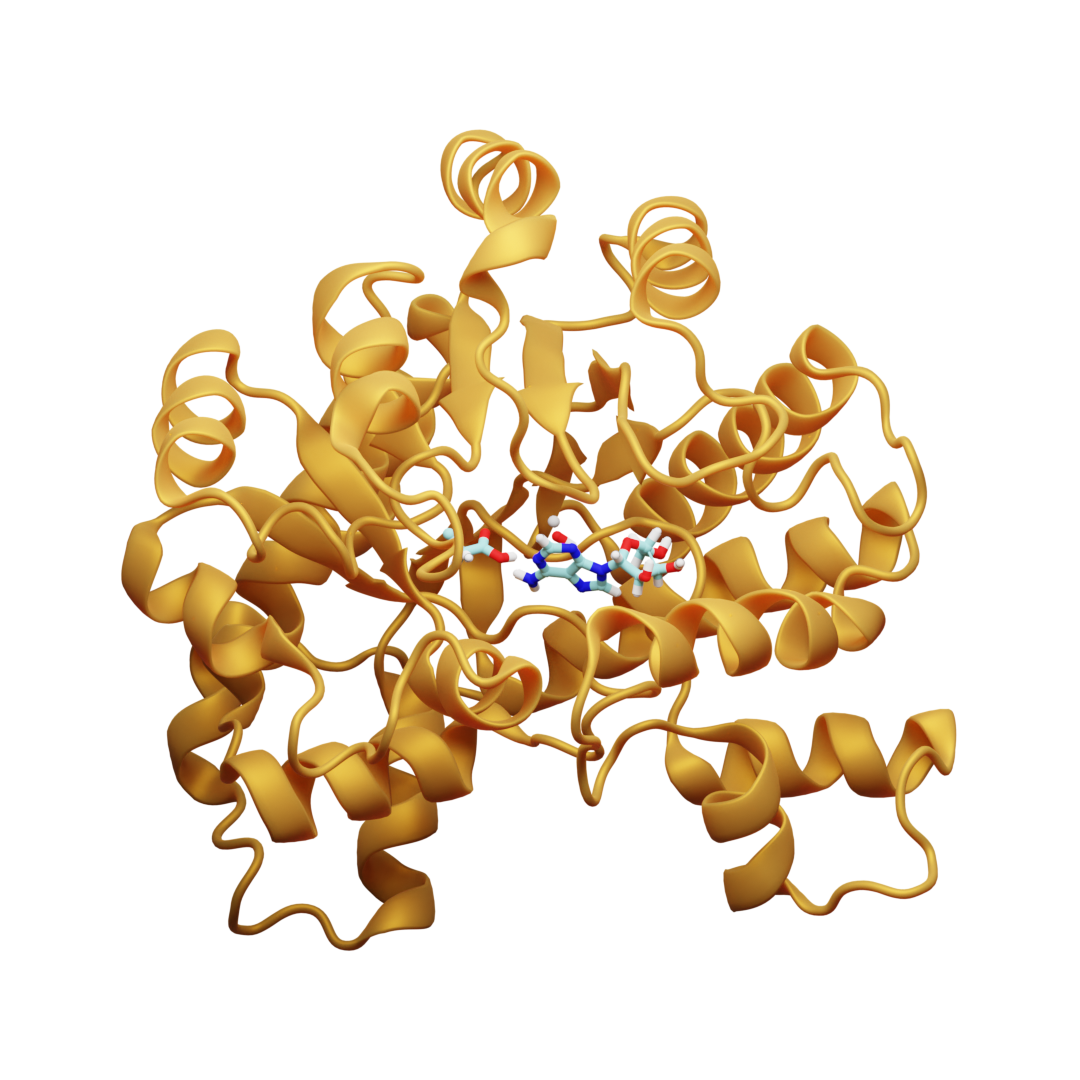
\includegraphics[scale=0.23]{figures/ada-equil.png}
\end{figure}
\end{frame}
%------------------------------------------------------------------------------
\begin{frame}
\frametitle{Free energies and comparison to experiments}
%\begin{minipage}{0.5\textwidth}
%\begin{figure}
%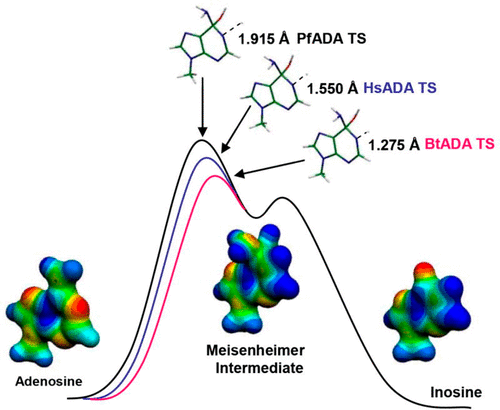
\includegraphics[scale=0.5]{figures/ada-exp.png}
%\end{figure}
%\end{minipage}
%\begin{minipage}{0.5\textwidth}
%\begin{figure}
%\centering
%\includegraphics[scale=0.5]{figures/ada-fenergy.pdf}
%\end{figure}
%\end{minipage}
\begin{figure}
   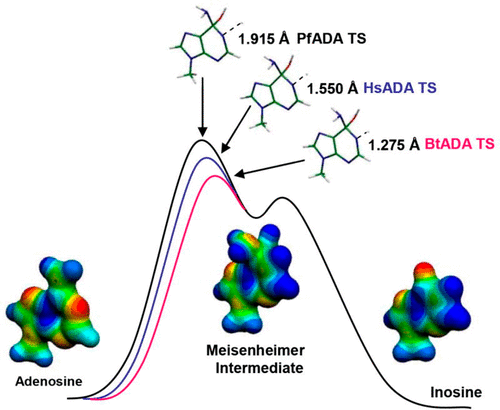
\includegraphics[width=0.475\textwidth]{figures/ada-exp.png}
   \hfill
   \includegraphics[width=0.475\textwidth]{figures/ada-fenergy.pdf}
\caption{Calculated free energy barrier: $21\;kcal\;mol^{-1}$}
\end{figure}
Qualitatively predicts the free energy profile as calculated from experiments for \textit{plasmodium falciparum}
adenosine deaminase.
\end{frame}
%------------------------------------------------------------------------------
\begin{frame}
\frametitle{Conclusions}
\begin{block}
{
    \begin{itemize}[<+-|alert@+>]
        \item  TPS based free energies are implemented 
        \item  Free energy calculations can be performed without the inclusion of 
        biasing potentials and the knowledge of reaction coordinates
        \item Free energy implementation was tested for the first time on enzyme catalyzed
        reactions, human MAT2A enzyme and plasmodium falciparum adenosine deaminase 
        \item The free energies calculated were qualitatively in good agreement with experimental
        measurements 
    \end{itemize}
}
\end{block}
\end{frame}
%------------------------------------------------------------------------------
\begin{frame}
\frametitle{Acknowledgements}
\begin{block}{Schwartz group}
\begin{itemize}
    \item Prof. Steven D. Schwartz
    \item Dr. Dimitri Antoniou
    \item Dr. Anthony Boldau
    \item Dr. Allison Smith
    \item Ananya Chakraborthy
    \item Bai Hei
    \item Clara Frost
    \item Dr. Elango Munusamy
\end{itemize}
\end{block}
\pause

\includegraphics[scale=0.1]{figures/nih-logo.png}
\end{frame}
%------------------------------------------------------------------------------
%\input{BeamerIntro.tex}
%\input{BeamerOverlays.tex}
%\input{funmath.tex}
%\input{BeamerConcl.tex}

\end{document}